%\documentclass[
  bibliography=totoc,     % Literatur im Inhaltsverzeichnis
  captions=tableheading,  % Tabellenüberschriften
  titlepage=firstiscover, % Titelseite ist Deckblatt
]{scrartcl}

% Paket float verbessern
\usepackage{scrhack}

% Warnung, falls nochmal kompiliert werden muss
\usepackage[aux]{rerunfilecheck}

% unverzichtbare Mathe-Befehle
\usepackage{amsmath}
% viele Mathe-Symbole
\usepackage{amssymb}
% Erweiterungen für amsmath
\usepackage{mathtools}

% Fonteinstellungen
\usepackage{fontspec}
% Latin Modern Fonts werden automatisch geladen
% Alternativ zum Beispiel:
%\setromanfont{Libertinus Serif}
%\setsansfont{Libertinus Sans}
%\setmonofont{Libertinus Mono}

% Wenn man andere Schriftarten gesetzt hat,
% sollte man das Seiten-Layout neu berechnen lassen
\recalctypearea{}

% deutsche Spracheinstellungen
\usepackage[ngerman]{babel}


\usepackage[
  math-style=ISO,    % ┐
  bold-style=ISO,    % │
  sans-style=italic, % │ ISO-Standard folgen
  nabla=upright,     % │
  partial=upright,   % │
  mathrm=sym,        % ┘
  warnings-off={           % ┐
    mathtools-colon,       % │ unnötige Warnungen ausschalten
    mathtools-overbracket, % │
  },                       % ┘
]{unicode-math}

% traditionelle Fonts für Mathematik
\setmathfont{Latin Modern Math}
% Alternativ zum Beispiel:
%\setmathfont{Libertinus Math}

\setmathfont{XITS Math}[range={scr, bfscr}]
\setmathfont{XITS Math}[range={cal, bfcal}, StylisticSet=1]

% Zahlen und Einheiten
\usepackage[
  locale=DE,                   % deutsche Einstellungen
  separate-uncertainty=true,   % immer Unsicherheit mit \pm
  per-mode=symbol-or-fraction, % / in inline math, fraction in display math
]{siunitx}

% chemische Formeln
\usepackage[
  version=4,
  math-greek=default, % ┐ mit unicode-math zusammenarbeiten
  text-greek=default, % ┘
]{mhchem}

% richtige Anführungszeichen
\usepackage[autostyle]{csquotes}

% schöne Brüche im Text
\usepackage{xfrac}

% Standardplatzierung für Floats einstellen
\usepackage{float}
\floatplacement{figure}{htbp}
\floatplacement{table}{htbp}

% Floats innerhalb einer Section halten
\usepackage[
  section, % Floats innerhalb der Section halten
  below,   % unterhalb der Section aber auf der selben Seite ist ok
]{placeins}

% Seite drehen für breite Tabellen: landscape Umgebung
\usepackage{pdflscape}

% Captions schöner machen.
\usepackage[
  labelfont=bf,        % Tabelle x: Abbildung y: ist jetzt fett
  font=small,          % Schrift etwas kleiner als Dokument
  width=0.9\textwidth, % maximale Breite einer Caption schmaler
]{caption}
% subfigure, subtable, subref
\usepackage{subcaption}

% Grafiken können eingebunden werden
\usepackage{graphicx}

% schöne Tabellen
\usepackage{tabularray}
\UseTblrLibrary{booktabs, siunitx}

% Verbesserungen am Schriftbild
\usepackage{microtype}

% Literaturverzeichnis
\usepackage[
  backend=biber,
]{biblatex}
% Quellendatenbank
\addbibresource{lit.bib}
\addbibresource{programme.bib}

% Hyperlinks im Dokument
\usepackage[
  german,
  unicode,        % Unicode in PDF-Attributen erlauben
  pdfusetitle,    % Titel, Autoren und Datum als PDF-Attribute
  pdfcreator={},  % ┐ PDF-Attribute säubern
  pdfproducer={}, % ┘
]{hyperref}
% erweiterte Bookmarks im PDF
\usepackage{bookmark}

% Trennung von Wörtern mit Strichen
\usepackage[shortcuts]{extdash}

\author{%
  Vincent Wirsdörfer\\%
  \href{mailto:vincent.wirsdoerfer@udo.edu}{authorA@udo.edu}%
  \and%
  Joris Daus\\%
  \href{mailto:joris.daus@udo.edu}{authorB@udo.edu}%
}
\publishers{TU Dortmund – Fakultät Physik}


%\begin{document}
\section{Versuchsdurchführung}
\label{sec:Versuchsdurchführung}

Zu Beginn des Versuches müssen divese Voraussetzungen geprüft werden, bevor die Wärmeleitfähigkeiten der Metalle experimentell untersucht werden können.
Dazu gehört beispielsweise die vollständige Verkabelung aller relevanten Geräte, sowie die korrekte Sensorik des Datenloggers. Außerdem muss der Abstand 
zweier benachbarter Thermoelemente gemessen werde, welche \textbf{nicht} durch das Peltierelement getrennt sind. Wie in \ref{fig:Versuchsaufbau} abgelesen werden kann,
ist das zum Beispiel der Abstand zwischen $T_1$ und $T_2$. 

\begin{figure}
    \centering
    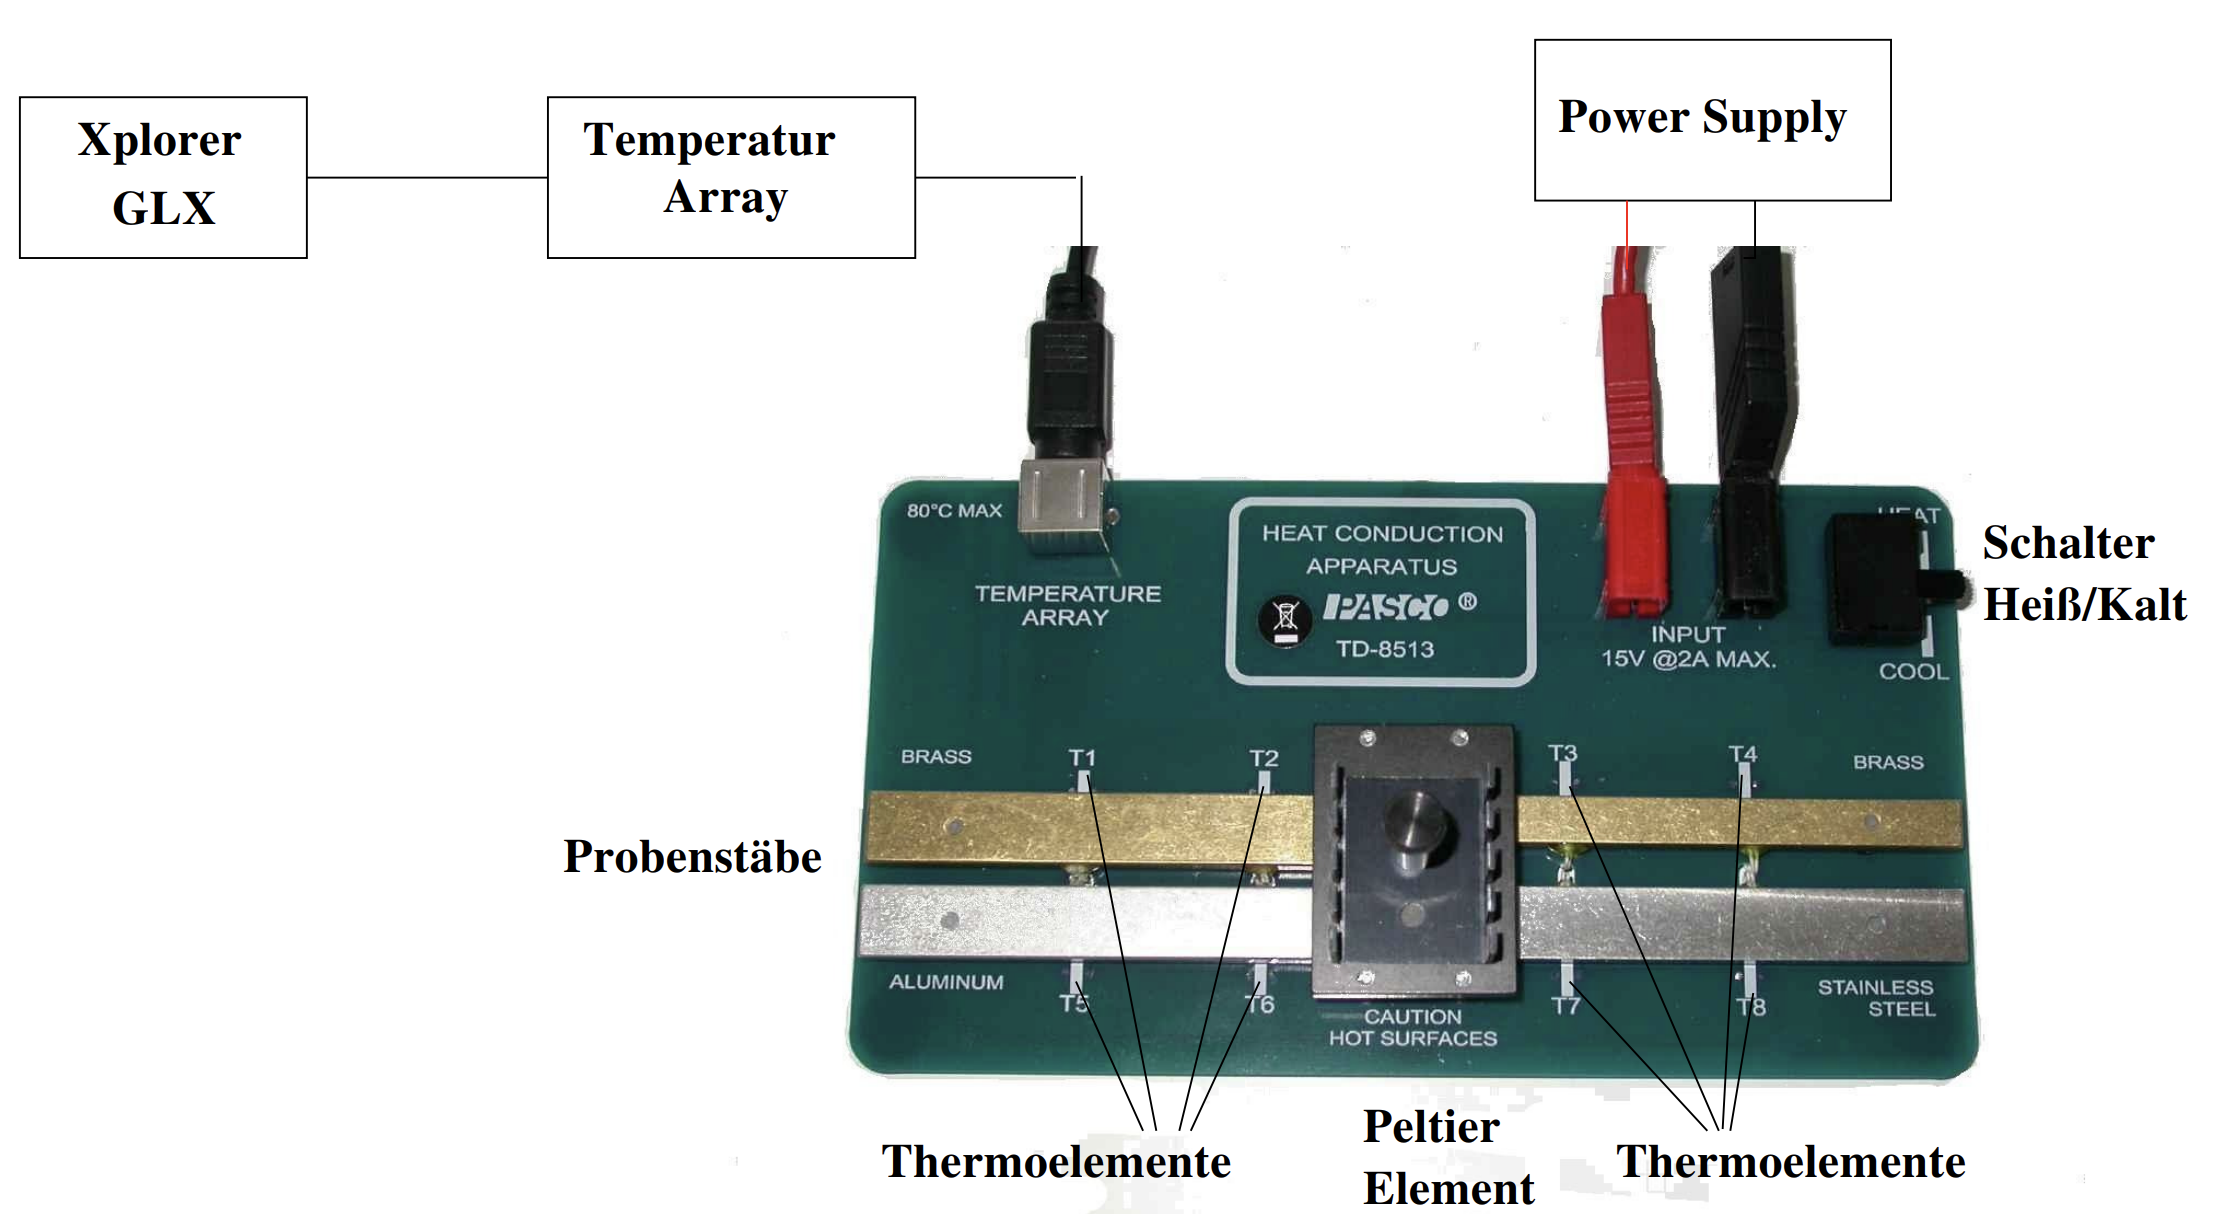
\includegraphics[width=\textwidth]{./content/Versuchsaufbau_v204.png}
    \caption{Versuchsaufbau}
    \label{fig:Versuchsaufbau}
\end{figure}

\subsection{Statische Methode}
\label{sec:Statische Methode}

Das Grundkonzept der statischen Methode besteht darin, den zeitlichen Verlauf der Temperaturänderung der jeweiligen Stäbe zu beobachten und so Rückschlüsse auf den
Wärmestrom $\sfrac{\increment Q}{\increment t}$ der Metalle zu ziehen. Dies gelingt, indem an jeweils zwei Stellen der Stäbe die Temperatur gemessen und schließlich als Funktion der Zeit aufgetragen wird. \\
Hierbei muss zunächst die Abtastrate des Datenloggers auf $\increment t_\text{GLX} = 10\,\unit{\second}$ eingestellt sein. Ferner wird die Spannung des Power Supplys bei maximaler Stromstärke auf 
$U_\text{P} = 5\,\unit{\volt}$ eingestellt. Sofern die Probestäbe der Grundplatte hinreichend abgekühlt sind\footnote{Die kann am Datenlogger unter Menüpunkt \texttt{Digital} eingesehen werden},
werden die Wärmeisolierungen an den Stäben angebracht. Im Anschluss kann der Schalter auf \enquote{HEAT} gestellt werden bis das Thermoelement $T_7$ auf eine Temperatur von 45\,\unit{\celsius}
erhitzt ist. Ist diese Schwelle erreicht, wird der Schiebeschalter erneut auf \enquote{COOL} umgestellt, die Wärmeisolierungen entfernt und die Probestäbe werden runtergekühlt. \\
Mittels des Menüpunktes \texttt{Tabellen} können nun die Temperaturwerte aller Thermoelemente zu den jeweiligen Zeitpunkten eingesehen werden. Folglich können somit die Werte der
sich fern vom Peltierelement befindenden Thermoelemente $T_1$, $T_4$, $T_5$ und $T_8$ nach ca. 700\,\unit{\second} notiert werden. Der komplette Datensatz wird extrahiert und auf einem USB-Stick
gesichert. Anhand dieser Daten können nun Temperaturverläufe der fernen Thermoelemente sowie der Temperaturdifferenzen $T_{7,8} = T_7 - T_8$ und $T_{2,1} = T_2 - T_1$ graphisch dargestellt werden.
Die Probestäbe werden so lange gekühlt, bis sich eine Temperatur von unter 30\,\unit{\celsius} einstellt.

\subsection{Dynamische Methode}
\label{sec:Dynamische Methode}

Die dynamische Methode (hier: \emph{Angström-Meßverfahren}) verfolgt den Ansatz, die Wärmeleitfähigkeit durch die Ausbreitungsgeschwindigkeit der Temperaturwelle zu bestimmen. Diese Welle
wird durch periodisches Erhitzen und Abkühlen der Probestäbe erzeugt. \\ Im Gegensatz zur statischen Methode wird nun die Abtastrate auf $\increment t_\text{GLX} = 2\,\unit{\second}$ gesetzt.
Außerdem wird am Power Supply nun eine Spannung von $U_\text{P} = 8\,\unit{\volt}$ angelegt. Zu Beginn wird eine Messung durchgeführt, wobei der Schalter abwechselnd 40\,$\unit{\second}$ auf \enquote{HEAT} und danach 40\,$\unit{\second}$ auf \enquote{COOL} steht. Insgesamt ergibt dies somit eine 
Periodendauer der Temperaturwelle von 80\,$\unit{\second}$. Dieser Vorgang wird für mindestens 10 Perioden wiederholt und die Stäbe im Anschluss erneut abgekühlt. Die daraus gewonnenen Daten können somit erneut extrahiert
und gesichert werden. Folglich können die Temperaturverläufe des breiten Messingstabes visualisiert und ausgewertet werden. Wenn die Probestäbe wieder hinreichend abgekühlt sind, erfolgt die zweite Messung.
Dabei bleibt der Ansatz der periodischen Erhitzung gleich, es ändert sich jedoch die Periodendauer der Temperaturwelle. Nun wird jeweils 100\,$\unit{\second}$ erhitzt und abgekühlt, was eine Periodendauer von
{200\,$\unit{\second}$} ergibt. Sobald eins der acht Thermoelemente eine Temperatur von 80\,$\unit{\celsius}$ erreicht, wird die Messung beendet. Letztlich werden die daraus entstandenen Daten gespeichert und dazu verwendet, 
den Temperaturverlauf von Edelstahl darzustellen und zu analysieren.

%\end{document}

